Single crystals show a nicely ordered, clean surface - two properties important for reliable and reproducible experiments. We have chosen both silver and copper as substrates. They form fcc lattices and their surface termination can be chosen by precise cutting along a symmetry plane of choice. For the course of this thesis, experiments are conducted mainly on (111) and (100) terminated surfaces.\footnote{See \cite{riemann_ionic_2002} for another examples of vicinal metal surfaces (531), (532), (221), (311), (211).} Commercially available, single crystals guarantee a high precision in facet orientation and purity (99.999 \%) \cite{mateck}. Remaining contaminations in copper (Ag: \SI{0.8}{ppm}, Pb: \SI{0.3}{ppm}, Bi: \SI{0.8}{ppm}) and silver (Cu: \SI{2}{ppm}, Fe: \SI{2}{ppm}, Au: \SI{0.8}{ppm}, Ni: \SI{0.8}{ppm}) are removed by repeated sputter and anneal cycles in UHV. Typical cool down temperatures $\leq 2 \frac{K}{s}$ result in a smooth, atomically flat surface with large terrace size.

\begin{table}
\centering
\caption{Inter atomic distances for Cu and Ag with respect to different surface termination. $a$ denotes the lattice constant and $\beta= \SI{60}{\degree}$ the angle within the (111) unit cell}
  \begin{tabular}{ccccc}
& Lattice constant a [\SI{}{\angstrom}] & Nearest neighbors [\SI{}{\angstrom}] & diagonal [\SI{}{\angstrom}]\\ \hline 
\multicolumn{2}{c}{fcc(100)} & $\frac{\sqrt{2}a}{2}$ & a \\
  Cu	 	& 3.61	& 2.55 | 2.55 & 3.61  \\
  Ag		& 4.09	& 2.89 | 2.89 & 4.09 \\ \hline 
\multicolumn{2}{c}{fcc(111)} & $\frac{\sqrt{2}a}{2} \ <110>$ & $\sqrt{2}a\sin(\frac{\beta}{2})$ | $\sqrt{2}a\cos(\frac{\beta}{2})$\\
Cu 		& 3.61	& 2.55 | 2.55	& 2.55 | 4.42 \\
Ag		& 4.09	& 2.89 | 2.89	& 2.89 | 5.01 \\ \hline
%
%\multicolumn{2}{c}{fcc(110)} & $\frac{\sqrt{2}a}{2}$ | a & $\sqrt{\frac{3}{2}}a$\\
%  Cu	 	& 3.61	& 2.55 | 3.61	& 4.42 \\
%  Ag		& 4.09	& 2.89 | 4.09	& 5.00 \\ \hline 
 \end{tabular}
\end{table}

\begin{figure}\centering
	\subfigure[(111)]{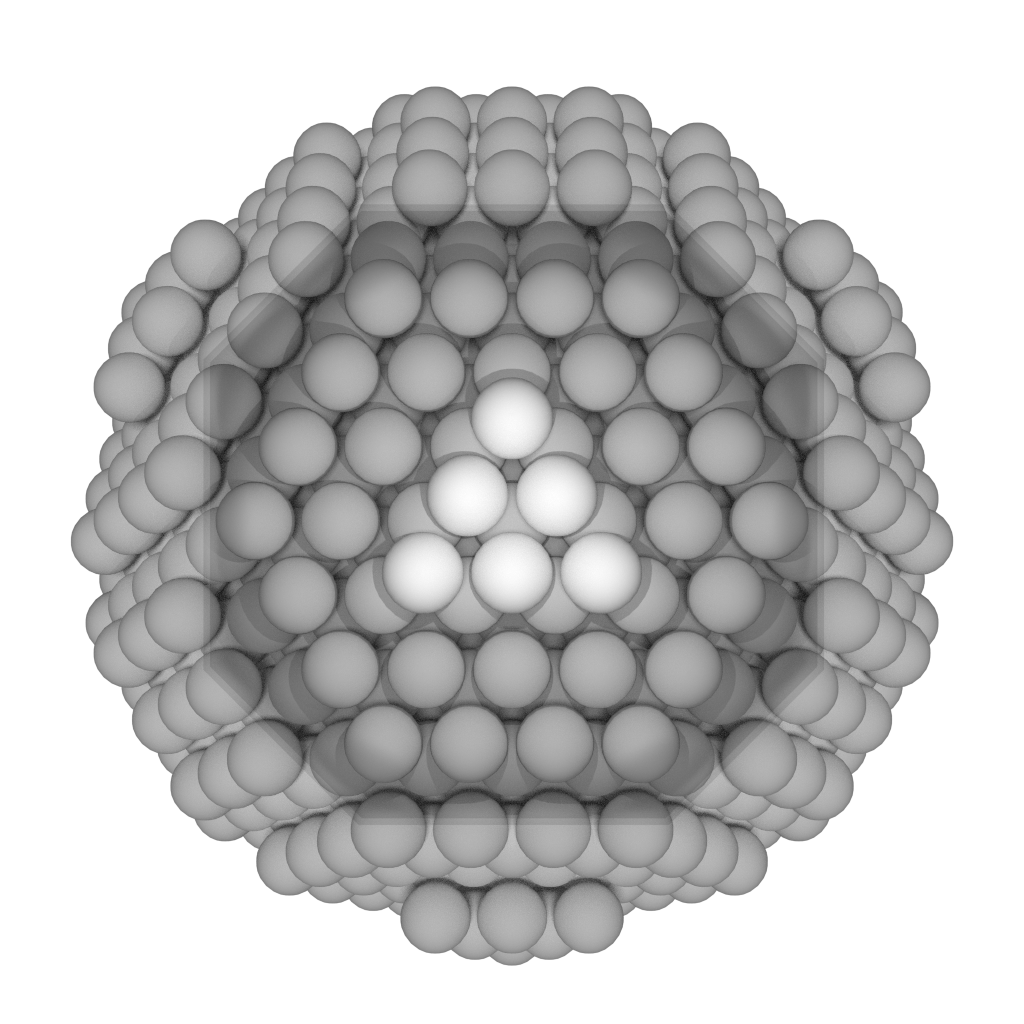
\includegraphics[width=0.3\textwidth]{./images/fcc-111-persp}}
	\subfigure[(100)]{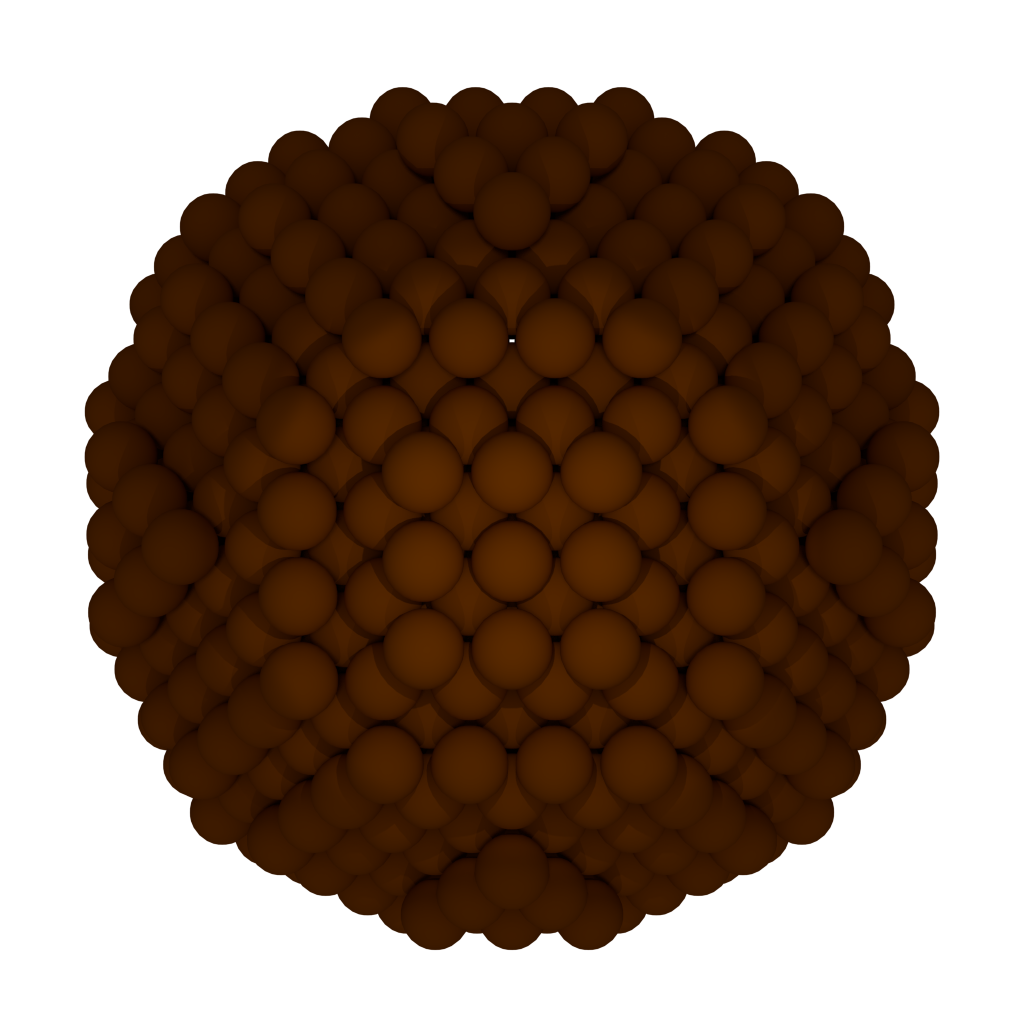
\includegraphics[width=0.3\textwidth]{./images/fcc-100-persp}}
%	\subfigure[(110)]{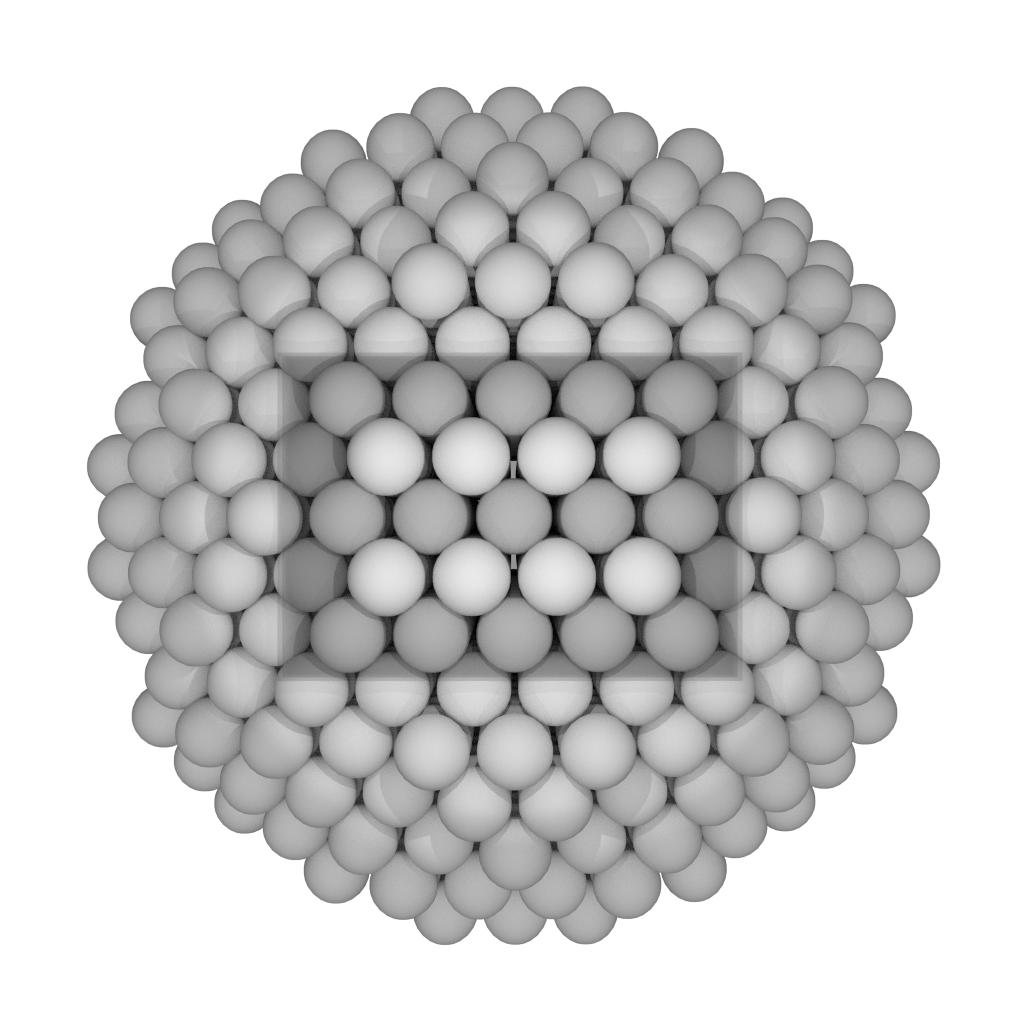
\includegraphics[width=0.3\textwidth]{./images/fcc-110-persp}}
	\caption{Identical crystalline balls in fcc lattice configuration. The surface termination is determined by the direction of the intersecting plane (parallel to the paper plane) relative to the lattice.}
	\label{fig:crystal-termination}
\end{figure}

 Dense packed rows are for fcc(111) the following directions: $<\bar 1 01>$, $<01\bar 1>$, $<1\bar 1 0>$. The diagonals are found in the $<\bar 1 \bar 1 2>$ and $<1\bar 2 1>$ directions. \underline{ADD INFO	FOR 100!!!}
 
% ``This surface consists of (111) terraces (three close-packed rows wide) and intrinsic (100) steps, which run parallel to the [011] direction. The close-packed atom rows located at the step edges are characterized by
%a nearest-neighbor distance of \SI{2.55}{\angstrom}  for Cu and of \SI{2.89}{\angstrom} for Ag, whereas the intrinsic step
%spacing is \SI{6.25}{\angstrom} for Cu and \SI{7.08}{\angstrom} for Ag. The surface symmetry is described by a primitive
%rectangular unit cell (cf. Figure 3.1a). The (111) terraces and the micro facets which represent the intrinsic (100) steps are tilted by \SI{19.5}{\degree}, respectively, to macroscopic (211) surface, which can be seen in the side view of the hard-sphere model in the upper panel of Figure 3.1a. The interlayer spacing for this surface is \SI{0.74}{\angstrom} for Cu and \SI{0.83}{\angstrom} for Ag.''
%
%``The (311) surface consists also of (111) terraces (two close-packed rows wide) and intrinsic (100) steps.''

Some experiments are done on polycrystalline surfaces of a copper foil. Here the surface termination is not homogeneous and is made of several domains with different facet orientation thus showing different step heights as indicated in table \ref{tab:step-heights}
\begin{table}\centering
\caption{Crystal properties from \cite[29ff]{riemann_ionic_2002, ma_interplay_2016, liu_oxygen_2014}}
\label{tab:step-heights}

\begin{tabular}{cccc}
			&				& Copper 	 & Silver \\
\multicolumn{2}{c}{Lattice constant}			& \SI{3.61}{\angstrom} & \SI{4.08}{\angstrom} \\
\multicolumn{2}{c}{Nearest neighbor}			& \SI{2.55}{\angstrom} & \SI{2.89}{\angstrom} \\ \hline \\
\multirow{3}{*}{Step height}	& (311) & \SI{4.23}{\angstrom} & \SI{4.78}{\angstrom} \\
								& (211) & \SI{6.25}{\angstrom} & \SI{7.07}{\angstrom} \\
								& (221) & \SI{7.66}{\angstrom} & \SI{8.65}{\angstrom} \\
								& (110) & \SI{1.38}{\angstrom} & \\
								& (111) & \SI{1}{\angstrom} & \\
								& (100) & \SI{1.8}{\angstrom} & \\

\end{tabular}
\end{table}

The surface free energy increases from the (111) surface with increasing angle of the (hkl) planes of interest with $$\cos(\phi)=\frac{h+k+l}{\sqrt{3(h^2+k^2+l^2)}}$$ \cite{jian-min_calculation_2004}. Thus, the (111) surface is the one with lowest energy, followed by (110) and (100).

\subsection{Dislocation lines and crystal orientation}
Due to the fact, that dislocation lines move within the crystal in a well defined manner, one can determine the crystals orientation when the orientation of a dislocation is known.
For fcc crystals the orientation of dislocation lines occurs in the {111} plane in $<110>$ direction. Its Burgers vector is $\frac{a}{2}[110]$\cite{_dislocation-theory}. \underline{ADD INFO	FOR 100!!!}